\documentclass{beamer}

\usepackage{tikz}
\usetheme{metropolis}

%\setbeamertemplate{frametitle}
%{\begin{centering}\smallskip
%	\insertframetitle\par
%\smallskip\end{centering}}
%\setbeamertemplate{itemize item}{$\bullet$}
%\setbeamertemplate{navigation symbols}{}
%\setbeamertemplate{footline}[text line]{%
%	\hfill\strut{%
%		\scriptsize\sf\color{black!60}%
%\quad\insertframenumber
%}%
%\hfill
%}
%
%% Define some colors:
%\definecolor{DarkFern}{HTML}{407428}
%\definecolor{DarkCharcoal}{HTML}{4D4944}
%\colorlet{Fern}{DarkFern!85!white}
%\colorlet{Charcoal}{DarkCharcoal!85!white}
%\colorlet{LightCharcoal}{Charcoal!50!white}
%\colorlet{AlertColor}{orange!80!black}
%\colorlet{DarkRed}{red!70!black}
%\colorlet{DarkBlue}{blue!70!black}
%\colorlet{DarkGreen}{green!70!black}
%
%% Use the colors:
%\setbeamercolor{title}{fg=Fern}
%\setbeamercolor{frametitle}{fg=Fern}
%\setbeamercolor{normal text}{fg=Charcoal}
%\setbeamercolor{block title}{fg=black,bg=Fern!25!white}
%\setbeamercolor{block body}{fg=black,bg=Fern!25!white}
%\setbeamercolor{alerted text}{fg=AlertColor}
%\setbeamercolor{itemize item}{fg=Charcoal}
%

\title{Some random beamer}
\subtitle{Yes, there is a lot you can do (and do)}
\author{Murray Heymann}
\institute{University of Stellenbosch}
\date{today}

\definecolor{USmaroon}{rgb}{0.55555, 0.058888, 0.17}
\usecolortheme[named=USmaroon]{structure}


\setbeamertemplate{navigation symbols}{}

\pgfdeclareimage[height=1cm]{university-logo}{uslogo.pdf}
\logo{\pgfuseimage{university-logo}}

\setbeamertemplate{bibliography item}{\insertbiblabel}

\begin{document}


\begin{frame}
	\titlepage
\end{frame}

\section{Everything is awesome}

\begin{frame}
	\frametitle{There is no largest prime}
	\framesubtitle{This proof uses \emph{reduction ad absurdum}}

	\begin{theorem}
		There is no largest prime number
	\end{theorem}


	\begin{proof}
		\begin{itemize}
			\item<1->
				Suppose $P = \{p_{1}, p_{2}, \dotsc, p_{r}\}$ are all the
				primes
			\item<2-3>
				Let $q = p_{1} p_{2} \dotsb p_{r}$
			\item<3> Let $p$ be a prime dividing $q+1$
			\item<4-> The $p \not \in P$, since then we would have $p \mid (q + 1 - q)$
			\item<1-> So $P$ cannot be all the primes
		\end{itemize}
	\end{proof}
\end{frame}

\section{Lord of the rings}

\begin{frame}
	\frametitle{Another one}
	\framesubtitle{let's have a look}


	\begin{itemize}
		\item
			One Ring to rule them all
		\item
			One Ring to find them
		\item
			One Ring to bring them all
		\item
			And in the darkness bind them
	\end{itemize}
\end{frame}

\begin{frame}
	\frametitle{T\textit{i}kZ}
	\framesubtitle{T\textit{i}kZ ist kein Zeichnungprogram}
\end{frame}
\begin{frame}
	\frametitle{T\textit{i}kZ}
	\url{texample.net}

	\begin{figure}
		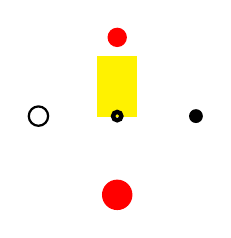
\begin{tikzpicture}[scale=0.5]
		\fill[yellow,draw] (-0.5,0) rectangle (0.5,1.5);
			\draw[ultra thick] (0,0) circle (3pt);
			\draw[thick] (-2, 0) circle(7pt);
		\fill (2,0) circle (5pt);
		\fill[red] (0, 2) circle (7pt)
				   (0,-2) circle (11pt);
	\end{tikzpicture}
		\caption{A T\textit{i}kZ drawing}
	\end{figure}
\end{frame}

\begin{frame}
	\frametitle{Connecting things}

	\begin{figure}
		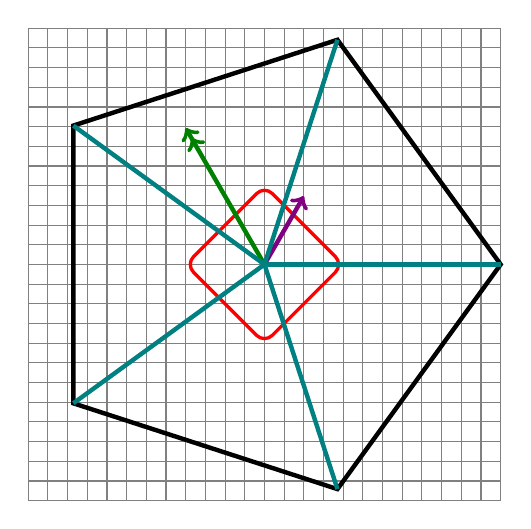
\begin{tikzpicture}
			\draw[step=0.25, color=gray] (-3,-3) grid (3,3);
			\draw[very thick, red, rounded corners]
				(1,0) -- (0, 1) -- (-1, 0) -- (0, -1) -- cycle;
			% color mixing below:  50 % blue, complement red
			\draw[ultra thick, blue!50!red, ->] 
				(0,0) -- (60:1cm);
			\draw[ultra thick, green!50!black, ->>] (0,0) -- (120:2cm);
			\path (0:3cm) coordinate (P0);
			\path (1*72:3cm) coordinate (P1);
			\path (2*72:3cm) coordinate (P2);
			\path (3*72:3cm) coordinate (P3);
			\path (4*72:3cm) coordinate (P4);
			\draw[ultra thick] (P0) -- (P1) -- (P2) -- (P3) -- (P4) -- cycle;
			\foreach \i in {0,...,4}
				\draw[ultra thick, blue!50!green] (0,0) -- (P\i);
		\end{tikzpicture}
		\caption{bla\cite{boom}}
	\end{figure}
\end{frame}

\begin{frame}
	\frametitle{Playing with nodes}
	
	\begin{figure}
		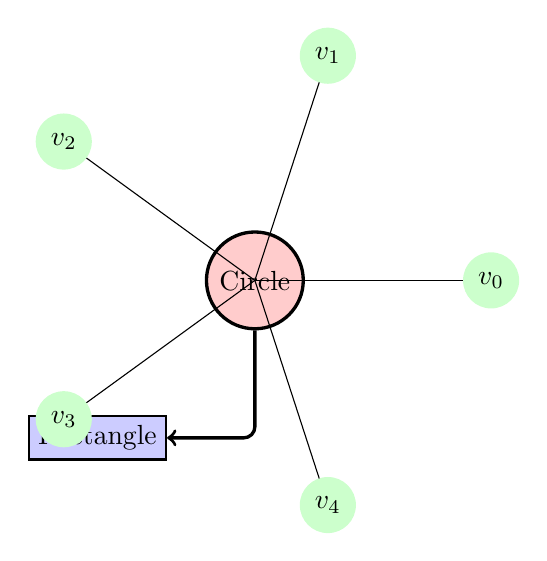
\begin{tikzpicture}
			\node[circle, fill=red!20, draw, very thick]
				(c1) at (0, 0) {Circle};
			\node[rectangle, fill=blue!20, draw, thick]
				(r1) at (-2, -2) {Rectangle};
			\draw[very thick, ->, rounded corners] (c1) -- (c1|-r1) -- (r1);
			\foreach \i in {0,...,4}
				\draw (0,0) -- (\i*72:3cm) node [fill=green!20, circle] (v\i) {$v_{\i}$};
		\end{tikzpicture}
		\caption{Nodes}
	\end{figure}
\end{frame}

\begin{frame}
	\frametitle{Scope}

	\begin{figure}	
		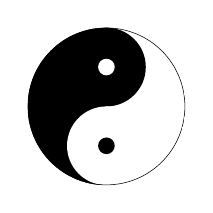
\begin{tikzpicture}
			\clip(0,0) circle (1cm);
			\fill[black] (0, 1) rectangle (-1, -1);
			\fill[black] (0, 0.5) circle (0.5cm);
			\fill[white] (0, -0.5) circle (0.5cm);
			\fill[white] (0, 0.5) circle (3pt);
			\fill[black] (0, -0.5) circle (3pt);
			\draw (0,0) circle (1cm);
		\end{tikzpicture}
		\caption{An illustration of scope.}
	\end{figure}	
\end{frame}

\begin{frame}
	\frametitle{Curved connections}

	\begin{figure}
		\begin{tikzpicture}
			\draw (0,0) .. controls (1,5) and (-4, -1) .. (7,1);
			\fill[red] (0,0) circle (2pt)
					   (7,1) circle (2pt);
			\fill[blue] (1,5) circle (2pt)
						(-4,-1) circle (2pt);

			\draw[green] (0:1cm) -- (0: 2cm) arc(0:60:2cm) -- 
				  (60:1cm) arc(60:0:1cm) -- cycle;
		\end{tikzpicture}
		\caption{Curved connections.}
	\end{figure}
\end{frame}

\begin{frame}
	\begin{tikzpicture}
		\draw plot file{sin.out};
		\draw[->] (-1, 0) -- (7, 0);
		\draw[->] (0, -1) -- (0, 2);
	\end{tikzpicture}

\end{frame}

\begin{frame}
	\frametitle{References}
	\begin{thebibliography}{1}
		\bibitem{koblitz} Kobliz
		\bibitem{boom} Boom
	\end{thebibliography}
\end{frame}

\end{document}
